\documentclass[../main.tex]{subfiles}

\begin{document}

Reference: [Borel, Automorphic forms on $\SL_2(\mathbb R)$]

$N=\left\{\begin{bmatrix}
1&*\\
0&1
\end{bmatrix}\right\}\subseteq B=\left\{\begin{bmatrix}
*&*\\
0&*
\end{bmatrix}\right\} \subseteq G=\GL_2(\mathbb R)^+\supseteq G_1=\SL_2(\mathbb R)\supseteq K=\SO(2)$, $A=\left\{\begin{bmatrix}
*&0\\
0&*
\end{bmatrix}\right\}$, $B=NA$, Iwasawa decomposition: $G=NAK$. $\Gamma\leq G_1$ is a discrete subgroup, $\Vol(\Gamma\backslash G_1)<\infty$. $\alpha$ is a obvious map $\GL_2(\mathbb R)\to\mathbb{CP}^1$

\begin{definition}[Siegel set]
For $a=\begin{bmatrix}
a_1&0\\
0&a_2
\end{bmatrix}\in A$, $\alpha(a)=\frac{a_1}{a_2}=\Im(a\cdot i)$, $\forall t>0$, let $A_t=\{a\in A|\alpha(a)>t\}$. Suppose $\infty\in P_\Gamma$ is a cusp of $\Gamma$, then $\Gamma\cap N=\left\langle\begin{bmatrix}
1&h\\
0&1
\end{bmatrix}\right\rangle\cong\mathbb Z$, for some $h>0$. Siegel sets at $\infty$ are of the form $S_t=\Omega A_tK$, $t>0$, $\Omega\subseteq N$ is a compact subset containing an interval of length $h$. In general, for a cusp $s=\sigma\infty$, Siegel sets at $s$ are $S_t=\sigma\Omega A_t\sigma^{-1}K$
\begin{center}
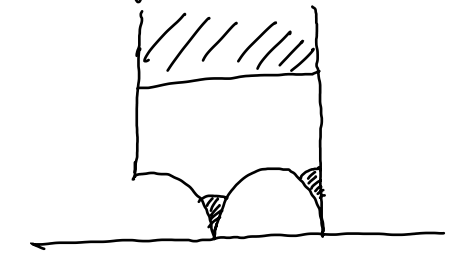
\includegraphics[scale=0.3]{Pictures/Siegel_set.png}
\end{center}
Let $\Gamma\backslash P_\Gamma=\{s_1,\cdots,s_n\}$, One can find Siegel sets $S_i$ at each cusp $s_i$ and a compact mod center set $C\subseteq G$ suc that $C\cup\bigcup_{i=1}^nS_i$ is a fundamental domain for $\Gamma\backslash G$
\end{definition}

\begin{definition}[Growth conditions]
Suppose $\infty\in P_\Gamma$, a function $\phi:\Gamma\backslash G\to\mathbb C$ has moderate growth at $\infty$ if $\exists $ Siegel set $S_t=\Omega A_t K$ and $\lambda\in\mathbb R$ such that $\phi(g)<<\Im(g\cdot i)^\lambda$, $\forall g\in S_t$. If this holds for all $\lambda\in\mathbb R$, we say $\phi$ has rapid decay at $\infty$. In general, for a cusp $s=\sigma\infty\in P_\Gamma$, we say $\phi$ has moderate growth/repid decay at $s$ if the function $\phi_\sigma(g)=\phi(\sigma g)$ is so at $\infty\in P_{\sigma^{-1}\Gamma\sigma}$
\end{definition}

\begin{proposition}\label{phi moderate growth at all cusps <=> phi moderate growth on G}
$\phi$ has moderate growth at all cusps of $\Gamma\iff\phi$ has moderate growth on $G$(as defined last time), see [Borel-5.11]
\end{proposition}

\begin{definition}
$\omega:Z_G\to\mathbb C^\times$ is a unitary character, define
\[L^2(\Gamma\backslash G,\omega)=\left\{f:\Gamma\backslash G\to\mathbb C|f(zg)=\omega(z)f(g),\forall z\in Z_G,\|f\|_2=\int_{\Gamma\backslash G/Z_G}|f|^2<\infty\right\}\]
\end{definition}

\begin{proposition}\label{|f*phi(g)|<<_phi Im(gi)|f|_2}
Suppose $\infty\in P_\Gamma$, let $\phi\in C_c(G)$, $t>0$, then $|f*\phi(g)|<<_\phi\Im(gi)\|f\|_2$, $\forall g\in NA_tK$, $f\in L^2(\Gamma\backslash G,\omega)$
\end{proposition}

\begin{proof}
Let $C\subseteq G$ be a compact subset such that $C^{-1}=\Supp\phi$, then
\[|f*\phi(g)|=|\int_Gf(gx)\phi(x^{-1})dx|\leq\|\phi\|_\infty\int _{gC}|f|\]
Let $g\in\lambda\begin{bmatrix}
1&x\\
0&1
\end{bmatrix}\begin{bmatrix}
y^{\frac{1}{2}}&0\\
0&y^{-\frac{1}{2}}
\end{bmatrix}K$, $y=\Im(gi)>t$. Let $C_N\subseteq N$, $C_A\subset A$ closed intervals such that $KC\subseteq C_NC_AK$
Then $gC\subseteq\lambda\begin{bmatrix}
1&x\\
1&1
\end{bmatrix}y^{-\frac{1}{2}}\begin{bmatrix}
y&0\\
0&1
\end{bmatrix}C_NC_AK=\lambda y^{-\frac{1}{2}}\begin{bmatrix}
1&x\\
1&1
\end{bmatrix}(ad\begin{bmatrix}
y&0\\
0&1
\end{bmatrix}C_N)\begin{bmatrix}
y&\\
0&1
\end{bmatrix}C_AK$. $ad\begin{bmatrix}
y&\\
0&1
\end{bmatrix}C_N$ scales $C_N$ by $y$, Need about $O(g)$ fundemantal domains to cover $gC$, $\int_{gC}|f|<<y\int_C|f|<<y\|f\|_1<<y\|f\|_2$

Constant term: Suppose $\infty\in P_\Gamma$, Let $\Gamma_N=\Gamma\cap N=\left\langle\begin{bmatrix}
1&h\\
0&1
\end{bmatrix}\right\rangle\cong\mathbb Z$, Let $\phi$ be a left $\Gamma _N$ invariant function on $G$
\[\phi_B(g)=\int_{\Gamma_N\backslash N}\phi(ng)dn\]
Then $\phi_B:N\backslash G\to\mathbb C$. For other cusps corresponding to conjugates $U\subseteq P$ of $N\subseteq B$, similarly, define $\phi_P:U\backslash G\to\mathbb C$
\end{proof}

Fundamental estimate [Borel-7.4]

\begin{lemma}\label{Lemma for fundamental estimate}
Let $f\in C^\infty(G)$ be left $\Gamma_N$ invariant, assume $\infty\in P_\Gamma$, let $X_1,\cdots,X_4\in\mathfrak g$ be an $\mathbb R$ basis, then $\exists c>0$ independent of $f$
\[|f(g)-f_B(g)|\leq c|\Im (gi)|^{-1}\sum_{j=1}^4|X_jf|_B(g),\forall g\in G\]
\end{lemma}

\begin{corollary}\label{A_0 subseteq L^2}
Any cusp form $\phi\in\mathcal A_0(\Gamma\backslash G,\chi,\omega)$ has rapid decay at all cusps. In particular, $|\phi|$ is bounded on $G$ and $\phi\in L^2(\Gamma\backslash G,\chi,\omega)$
\end{corollary}

\begin{proof}
Reduce to show rapid decay at $\infty\in P_\Gamma$, by assumption and Proposition \ref{phi moderate growth at all cusps <=> phi moderate growth on G}, $\phi(g)<< \Im(gi)^\lambda$ near $\infty$ for some exponent $\lambda\in\mathbb R$. Theorem \ref{Harish-Chandra theorem} $\Rightarrow$ $D\phi(g)<< \Im(gi)^\lambda$ near $\infty$, $\forall D\in U(\mathfrak g_{\mathbb C})$, same bound for $|D\phi|_B$. Take $D=X_j$ in Lemma \ref{Lemma for fundamental estimate}, recall $\phi_B=0$, get $\phi(g)<<\Im(gi)^{\lambda-1}\Rightarrow$ same for $D\phi$ and $|D\phi|_B$
Repeatedly apply Lemma \ref{Lemma for fundamental estimate} and Theorem \ref{Harish-Chandra theorem}, we get 
\[\phi(g)<<\Im(gi)^{\lambda-2},\cdots \Im(gi)^{\lambda-m},\forall m>0\]
near $\infty$, thus rapid decay
\end{proof}

\begin{definition}[$L^2$ cusp forms]
$L^2_0(\Gamma\backslash G,\chi,\omega)$ is the set of $\phi\in L^2(\Gamma\backslash G,\chi,\omega)$ such that for almost every $g$(except for a measure zero set) and any unipotent $U\subseteq G$ with $\Gamma\cap U\neq\{1\}$
$\int_{\Gamma\cap U\backslash U}\phi(ug)du=0$
\end{definition}

\begin{corollary}\label{f in L_0^2, |f*g(g)|<=c|f|_2}
Let $\phi\in C^\infty_c(G)$, then $\exists c>0$ such that forall $f\in L^2_0(\Gamma\backslash G,\chi,\omega)$, $|(f*\phi)(g)|\leq c\|f\|_2$, for all $g\in G$. Moreover, $f*\phi$ is rapidly decreasing near cusps
\end{corollary}

\begin{proof}
Suffices to prove this near all cusps, reduce to $\infty\in P_\Gamma$, by Proposition \ref{|f*phi(g)|<<_phi Im(gi)|f|_2}, $|f*\phi(g)|<<\Im(gi)\|f\|_2$ for $g$ near $\infty$
\[|D(f*\phi)(g)|=|f*D\phi(g)|<<\Im(gi)\|f\|_2,\forall D\in U(\mathfrak g_{\mathbb C})\]
Same for $|D(f*\phi)(g)|_B$. By assumption $(f*\phi)_B=f_B*\phi=0$. Apply Lemma \ref{Lemma for fundamental estimate} repeatedly $\Rightarrow f*\phi$ decrease rapidly at $\infty$
\end{proof}

\begin{proof}[proof of lemma \ref{Lemma for fundamental estimate}]
Fix $g\in G$, let 
\[\phi(t)=f(g)-f\left(\begin{bmatrix}1&t\\0&1\end{bmatrix} g\right)\]
then $\phi\in C^\infty(\mathbb R)$, $\phi(0)=0$, $\displaystyle\int_0^1\phi dt=f(g)-f_B(g)$, $\displaystyle|\phi(t)|\leq\int_0^1|\phi'|ds$, $|f(g)-f_B(g)|\leq\displaystyle\int_0^1|\phi|dt\leq\int_0^1|\phi'|dt$
Write $g=\lambda\begin{bmatrix}
1&x\\
0&1
\end{bmatrix}\begin{bmatrix}
y^{\frac{1}{2}}&0\\
0&y^{-\frac{1}{2}}
\end{bmatrix}k$, $k\in K$
\begin{align*}
\begin{bmatrix}
1&t+h \\
0&1
\end{bmatrix}g&=\begin{bmatrix}
1&t \\
0&1
\end{bmatrix}gg^{-1}\begin{bmatrix}
1&h \\
0&1
\end{bmatrix}g \\
&=\begin{bmatrix}
1&t \\
0&1
\end{bmatrix}gk^{-1}\begin{bmatrix}
1&h/y \\
0&1
\end{bmatrix}k \\
&=\begin{bmatrix}
1&t \\
0&1
\end{bmatrix}g\exp(h\ad(k)^{-1}(y^{-1}E))
\end{align*}
$E=\begin{bmatrix}
0&1\\
0&0
\end{bmatrix}$. Write $\ad(k)^{-1}E=\sum_{j=1}^4a_j(k)X_j$, $a_j:K\to\mathbb R$ are continuous and bounded
\begin{align*}
|\phi'(t)|&=\left|y^{-1}\sum_{j=1}^4a_j(k)(X_jf)\left(\begin{bmatrix}
1&t\\
0&1
\end{bmatrix}g\right)\right| \\
&\leq cy^{-1}\sum_{j=1}^4\left|X_jf\left(\begin{bmatrix}
1&t\\
0&1
\end{bmatrix}g\right)\right|
\end{align*}
$c=\max_{j,k}|a_j(k)|$ is independent of $f$
\[|f(g)-f_B(g)|\leq\int_0^1|\phi'(t)|dt\leq cy^{-1}\sum_{j=1}^4|X_f|_B(g)\]
\end{proof}

\end{document}